\begin{section}{Numeric results}
\label{Numerics}

\begin{subsection}{One dimensional system}

We will start with a one dimensional chain with hamiltonian $\hat{H} = \sum_{\langle i,j \rangle} |J_1| \bs{S}_i\bs{S}_j - \sum_{\langle \langle i,j \rangle \rangle} \nu_{ij}|D_2|\hat{e}_z\bs{S}_i \times \bs{S}_j$. This approximated Hamiltonian with no NNN exchange interaction is very simple, but in some systems where it has even been observed that $|\bs{D}_{2,ij}| > |J_{2,ij}|$ \cite{Chen2018} it can be a good approximation.  We write the absolute values in $|J_1|$ and $|D_2|$ to limit the analysis to the range in which the field does not change the sign of these factors. In this case we can write $\bs{S}(r) = S(\cos(kr), \sin(kr), 0)$, where the real number $k$ plays the role of the wavevector, and $\theta = ka-\pi$ is the deviation from the N\'eel state. This form assumes spiral order, with N\'eel state being the special case $\theta = 0$ (or $k = \pi$). From now we will use $\theta$ instead of $k$. Then the classical energy per site is given by:

\begin{equation}
\frac{E(\theta)}{2S^2} = -|J_1|\cos(\theta) - |D_2|\sin(2 \theta)
\end{equation}

and the energy is minimized for $\theta^* = \arcsin(\frac{-\frac{J_1}{D_2} + \sqrt{(\frac{J_1}{D_2})^2+32}}{8})$, i.e. $\theta^* = \theta^*(\frac{J_1}{D_2})$. This is the correct minimization for $J_1, D_2 > 0$. Next we will show numerically that the ratio between the NN and NNN parameters, $\frac{J_1}{D_2}$, can be modulated by the intensity of the field, and therefore the field can be used to control the SDW wavevector. 

We will use the time average approximation \ref{MFactorApprox0} so that we can write:

\begin{align}
J_{1,ij} &= J_{1,ij}^0  \sum_{n} \frac{\mathcal{J}_n(\alpha_{ij})^2}{1+n\frac{\omega}{\text{U}}} \\
D_{2,ij} &= D_{2,ij}^0  \sum_{n} \frac{\mathcal{J}_n(\alpha_{ij})^2}{1+n\frac{\omega}{\text{U}}}
\end{align}

Where $\bs{D}_{2,ij} = \hat{e}_z D_{2,ij}$ and where $J_{1,ij}^0 = J_{1}^0 = \frac{2t_1^2}{\text{U}}$ and $D_{2,ij}^0 = -\frac{4t_2\Delta\nu_{ij}}{\text{U}}$. Since $\mathcal{J}_n(-x) = (-1)^n\mathcal{J}_n(x)$ the dependance is on $|\alpha_{ij}|$ only. Now, using \ref{Def_alpha}, for circularly polarized light we have $|\alpha_{ij}| = \frac{1}{\sqrt{2}}e|\vec{R}_{ij}| \frac{E_0}{\omega} = \frac{1}{\sqrt{2}}ea \frac{E_0}{\omega} \frac{|\vec{R}_{ij}|}{a} = \frac{|\vec{R}_{ij}|}{\sqrt{2}a} \mathcal{E}$, where $a$ is the lattice constant and $\mathcal{E} = \frac{eaE_0}{\omega}$. Now, for $J_{1,ij}$, $i$ and $j$ are NN and so we can write $|\vec{R}_{ij}|=a$, whereas for $D_{2,ij}$, $i$ and $j$ are NNN and so $|\vec{R}_{ij}|=2a$. Thus:

\begin{align}
J_{1,ij} &= J_{1} = J_{1}^0  \sum_{n} \frac{\mathcal{J}_n(\frac{1}{\sqrt{2}}\mathcal{E})^2}{1+n\frac{\omega}{\text{U}}} \\
D_{2,ij} &= D_{2,ij}^0  \sum_{n} \frac{\mathcal{J}_n(\sqrt{2}\mathcal{E})^2}{1+n\frac{\omega}{\text{U}}}
\end{align}

In each case the absolute vale is independent of $i,j$.  Now, in units $\hbar=t_1=1$ we measure energy in units of $t_1$ and frequency in units of $\frac{t_1}{\hbar}$. Then, for $t_2 = 0.1$, $\Delta = 0.5$, $\text{U} = 10$ and $\omega = 6, 16$ we obtain the plots in Figure \ref{Fig3.1:NNvsNNN}. The ratio $\frac{J_{1,ij}}{D_{2,ij}}$ is plotted in Figure \ref{Fig3.1:ratio}. The field can change the sign of $J_1$ and $D_2$ for strong amplitudes. Finally, in Figure \ref{Fig3.2} we plot the SDW NN angle $\theta$ limited to the case $J_1 > 0$ and $D_2 > 0$.

\begin{figure}
\centering
\begin{subfigure}{.45\textwidth}
  %\centering
  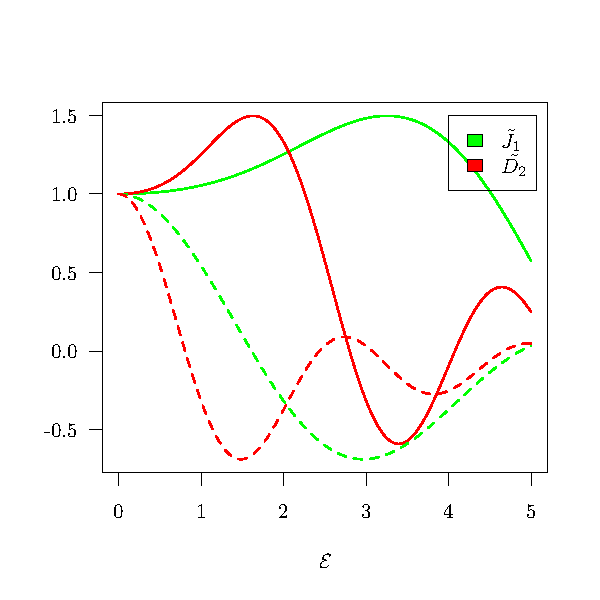
\includegraphics[width=1\linewidth]{Figures/NNvsNNN.pdf}
  \caption{$\frac{J_{1}}{J_{1}^0}$ and $\frac{D_{2,ij}}{D_{2,ij}^0}$ are plotted as function of $\mathcal{E}$. Similar results are obtained in \cite{Mentink2015} for $J_{1}$. Solid lines are for $\omega = 6$ and dashed lines are for $\omega = 16$.}
  \label{Fig3.1:NNvsNNN}
\end{subfigure}%
\hspace*{\fill}
\begin{subfigure}{.45\textwidth}
  %\centering
  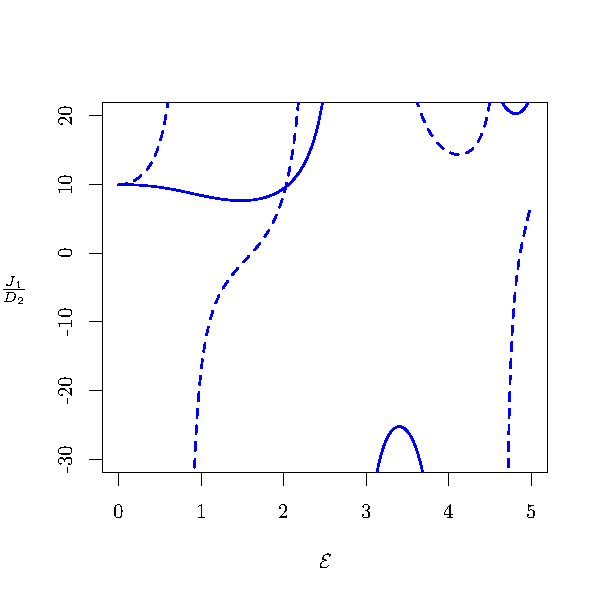
\includegraphics[width=1\linewidth]{Figures/ratio.pdf}
  \caption{$\frac{J_{1}}{D_{2,ij}}$ is plotted as function of $\mathcal{E}$, it diverges every time $D_{2,ij}$ changes sign. Solid lines are for $\omega = 6$ and dashed lines are for $\omega = 16$.}
  \label{Fig3.1:ratio}
\end{subfigure}
\label{Fig3.1}
\end{figure}

\begin{figure}
\centering
  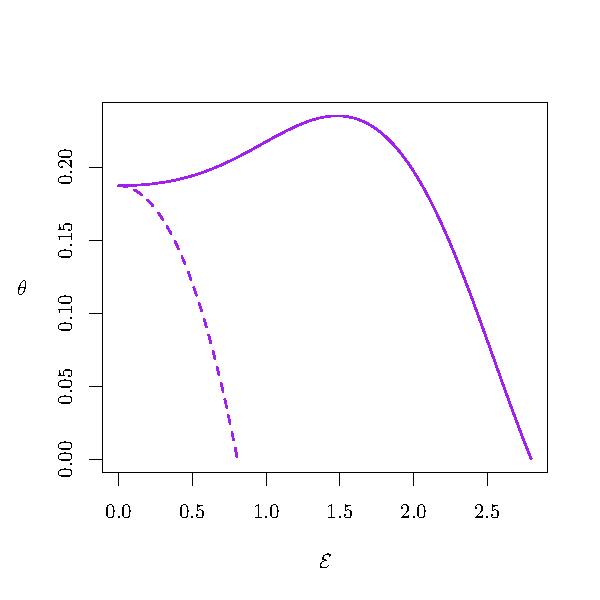
\includegraphics[width=0.5\linewidth]{Figures/theta.pdf}
  \caption{The spin wave density NN angle $\theta$ as a function of $\mathcal{E}$. The field modifies the ratio $\frac{J_{1}}{D_{2,ij}}$ thus modifying the wave vector. Solid lines are for $\omega = 6$ and dashed lines are for $\omega = 16$.}
\label{Fig3.2}
\end{figure}

\end{subsection}

\begin{subsection}{Two dimensional systems}
 
In a honeycomb lattice described by the effective spin model \ref{MKMHeff} the usual approach is to write:

\begin{align}
\bs{S}_1(\bs{r}) &= S\left( \cos(\bs{Q}\bs{r}), \sin(\bs{Q}\bs{r}), 0 \right) \\
\bs{S}_2(\bs{r}) &= -S\left( \cos(\bs{Q}\bs{r} + \theta), \sin(\bs{Q}\bs{r} + \theta), 0 \right)
\end{align}

The $1, 2$ subindex stands for the sublattice. The $\hat{e}_z$ component vanishes in order to minimize the contribution of the pseudodipolar interaction. Let $Q_a = \bs{Q}\hat{\bs{a}}$ and $Q_b = \bs{Q}\hat{\bs{b}}$, where $\hat{\bs{a}}$ and $\hat{\bs{b}}$ are the primitive cell vectors. Then, the classical energy per spin is given by:

\begin{align}
\frac{E}{NS^2} &= -\frac{J_1}{2}\left( \cos(\theta) + \cos(\theta - Q_a - Q_b) + \cos(\theta - Q_b) \right) + \nonumber \\
&+ (J_2-\Gamma) \left( \cos(Q_a) + \cos(Q_b) + \cos(Q_a+Q_b) \right)+ \nonumber \\
&+D_2\left( \sin(Q_a) + \sin(Q_b) + \sin(Q_a+Q_b) \right)
\end{align}

Notice that when the spins are constrained in the $\hat{e}_x, \hat{e}_y$ plane, the anisotropic interaction $\bs{S}_i\bs{\Gamma}_{ij}\bs{S}_j$ becomes a ferromagnetic interaction. The minimization of this energy will lead to an involved phase diagram in the $J_1, J_2, D_2, \Gamma_2$ space (or equivalently, in the $t_1, t_2, \Delta$ space). We will not attempt to describe this phase diagram. However, as we have shown in the one dimensional case, by modulating the laser amplitude we can control the ratio between the NN and NNN coupling factors, and thus the parameters $\bs{Q}$ and $\theta$ of the system state.

\end{subsection}

\end{section}
